%% Generates the placeholder images shipped with this template.
%% They exist only so the figure examples compile out of the box, and are
%% meant to be deleted once real figures replace them.
%%
%%   pdflatex placeholders.tex
%%   pdfseparate placeholders.pdf p-%d.pdf
%%
%% Page 1 becomes placeholder-a, page 2 placeholder-b, page 3
%% placeholder-wide.
%%
%% multi=tikzpicture puts each picture on a page of its own. The
%% environments have to appear literally in the body for it to see them,
%% so the drawing is factored into \panel rather than the environment.
\documentclass[border=0pt,multi=tikzpicture]{standalone}
\usepackage[T1]{fontenc}
\usepackage{newtxtext}   % Times, so the placeholders match manuscript.cls
\usepackage{tikz}

% #1 width, #2 height, #3 label
\newcommand{\panel}[3]{%
  \fill[black!10] (0,0) rectangle (#1,#2);
  \draw[black!25] (0,0) -- (#1,#2) (0,#2) -- (#1,0);
  \draw[black!40] (0,0) rectangle (#1,#2);
  \node[font=\Huge\bfseries, text=black!50] at (#1/2,#2/2+0.35) {#3};
  \node[font=\small, text=black!45] at (#1/2,#2/2-0.55)
    {placeholder, replace with a real figure};
}

\begin{document}

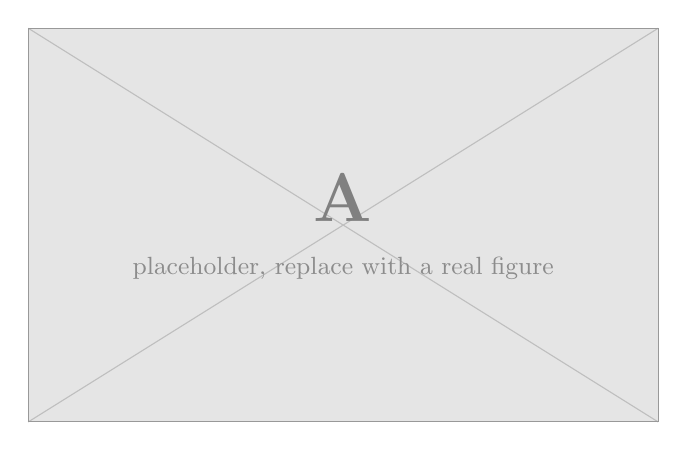
\begin{tikzpicture}
  \panel{8}{5}{A}
\end{tikzpicture}

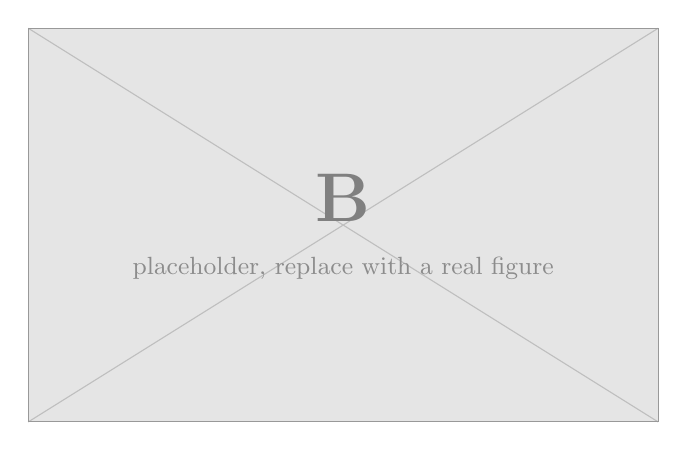
\begin{tikzpicture}
  \panel{8}{5}{B}
\end{tikzpicture}

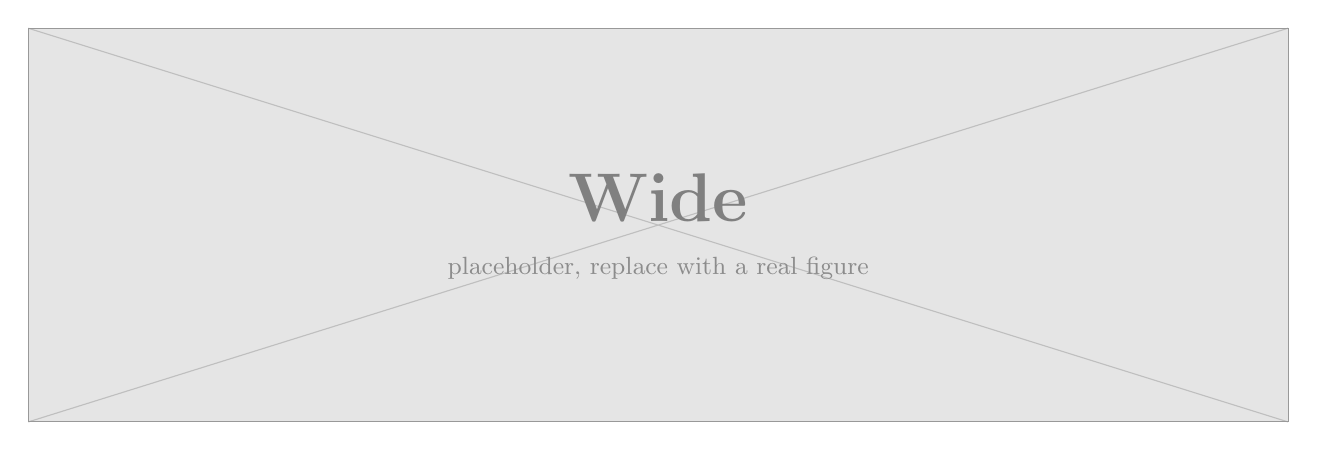
\begin{tikzpicture}
  \panel{16}{5}{Wide}
\end{tikzpicture}

\end{document}
